\capitulo{6}{Trabajos relacionados}

En este apartado vamos a ver varias herramientas que hacen uso del sentiment analysis.

\section{MonkeyLearn}
MonkeyLearn \cite{monkeylearn} es una aplicación que utiliza machine learning para analizar el texto. Puede integrarse con aplicaciones como Excel, Google Sheets, Zapier, Gmail, Twitter, etc. 

Además de poder utilizar su analizador de texto, te permite entrenarlo de forma personalizada añadiendo palabras que quieras destacar.

Respecto al precio, tiene tres planes diferentes:
\begin{itemize}
	
\item Un plan gratuito que está bastante reducido ya que te permite analizar 300 veces al mes, a baja velocidad y además no te permite ver los resultados en gráficos.
\item Un plan llamado “Team” que permite analizar hasta 10000 veces al mes con una velocidad media, se pueden definir hasta 3000 palabras nuevas para entrenar el algoritmo, pero tampoco nos permite mostrar los resultados en gráficos.
El precio es de 299\$ por mes.
\item Un plan llamado “Business” que es personalizado, nosotros nos encargaremos de decidir cuántas querys queremos analizar al mes, la velocidad de la aplicación, las palabras a definir. Además, los resultados se mostrarán en gráficos y flujogramas. 
El precio será variable.
\end{itemize}

\imagen{trabajos_relacionados/monkeylearn1}{Monkeylearn connect your text data.}

\imagen{trabajos_relacionados/monkeylearn2}{Monkeylearn turn your text into tags.}

\imagen{trabajos_relacionados/monkeylearn3}{Monkeylearn put your tags to work.}

\section{Lexalytics}
Es una aplicación que se basa en el Natural Language Processing para crear distintas librerías y modelos. Lexalytics \cite{lexalytics} también utiliza machine learning para entrenar a los modelos.

Además de utilizar sentiment analysis en los textos, los separan en categorías dependiendo del tema que se trate en el texto y extraen las distintas entidades como la persona que ha escrito, el lugar desde donde se escribe, los productos sobre los que se escriben, etc.

El precio de la aplicación es variable dependiendo de cuántos textos queramos analizar, el tiempo que vayamos a suscribirnos, etc. 

\begin{figure}[h]
    \advance\leftskip4cm 
    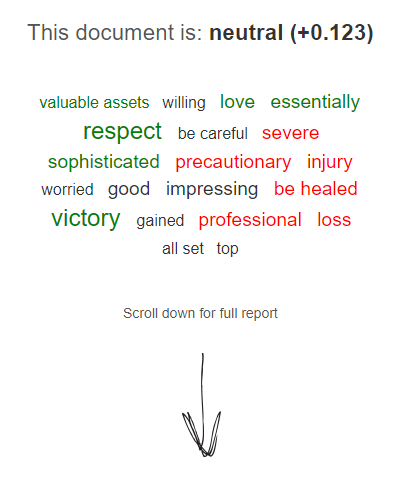
\includegraphics[scale=0.55]{trabajos_relacionados/lexalytics}
    \caption{Lexalytics análisis de texto}
\end{figure}


\imagen{trabajos_relacionados/lexalytics2}{Lexalytics entidades.}
\imagen{trabajos_relacionados/lexalytics3}{Lexalytics entidades subrayadas en el texto.}
\newpage
\section{Brandwatch}
Brandwatch \cite{brandwatch} es una aplicación que permite a las marcas saber que opina la gente sobre ellas en las redes sociales e internet mediante inteligencia artificial. 

Permite categorizar los datos y entrenar el modelo de forma personalizada añadiendo palabras que queramos que identifique como positivas o negativas en caso de estar en algún comentario.
Permite mostrar los datos recogidos en distintos tipos de gráficos y pudiendo personalizarlos para que muestre las categorías que queramos.

Además, nos permite analizar distintos perfiles de personas para poder realizar campañas de marketing que lleguen a las personas que queramos enfocar nuestra empresa.	

Los precios varían dependiendo de los planes:


\begin{table}[ht!]
    \centering
    \resizebox{15cm}{!} {
    \begin{tabular}{l l c}
    
         \textbf{Plan}    &\textbf{Descripción} &  \textbf{Precio } \\ \hline
         \textit{Brandwatch/Pro} &{Está orientado a analistas de marcas pequeñas}      & 653,59\$/mes \\ 
         \textit{Enterprise/M} &\parbox[p][0.2\textwidth][c]{8cm}{Para empresas de marcas algo más conocidas y por tanto con mayor volumen de opiniones}      & 2614,37\$/mes \\ 
         \textit{Enterprise/Q} &\parbox[p][0.2\textwidth][c]{8cm}{Orientado a empresas importantes y que tienen muchos comentarios que analizar}      & 2614,37\$/mes \\ 
    \end{tabular}}
    \caption{Precios de Brandwatch.}
    \label{tab:my_label}
\end{table}


Además cuentan con planes personalizados para agencias.

\imagen{trabajos_relacionados/brandwatch}{Brandwatch gráfico de líneas.}
\imagen{trabajos_relacionados/brandwatch2}{Brandwatch gráfico de burbujas.}
